\documentclass{article}
\usepackage{amsmath}
\usepackage[utf8]{inputenc}
\usepackage[T1]{fontenc}
\usepackage[ngerman]{babel}
\usepackage{amsfonts}
\usepackage[left=3cm,right=2cm,top=2.5cm,bottom=2cm]{geometry}
\usepackage{karnaugh-map}
\usepackage{tikz}
\usepackage{cancel}
% \usepackage{circuitikz}
\usepackage{kvmap}
\usepackage{subcaption}
\usepackage{placeins}
\usepackage[european,noarrowmos]{circuitikz}
% \usetikzlibrary{calc,intersections,shapes.gates.logic.IEC}

\title{Grundlagen der Rechnerarchitektur: Übungsblatt 6}
\author{Alexander Waldenmaier, Maryia Masla}

\begin{document}
    \maketitle
	\subsection*{Aufgabe 1: Quine McCluskey}
	\begin{enumerate}
		\newlength{\height}
		\setlength{\height}{2em}
		\newlength{\width}
		\setlength{\width}{3cm}
		\item[a)] Minimierung von $f$: \\\\
		\begin{tikzpicture}[baseline=(current bounding box.south)]
			\foreach \val[count=\i from 1, evaluate=\i as \j using int(\i+1)] in {
				$\overline{x_0}\overline{x_1}\overline{x_2}$,
				$\overline{x_0}x_1x_2$,
				$x_0 \overline{x_1} x_2$,
				$x_0 x_1 \overline{x_2}$,
				$x_0x_1x_2$
			}
			\node at(0\width, {-(\i-1)*\height})[] (A\i) {\i. \val};

			\foreach \val[count=\i from 1, evaluate=\i as \j using int(\i+1)] in {
				$x_1 x_2$,
				$x_0 x_2$,
				$x_0 x_1$
			}
			\node at(1\width, {-(\i-1)*\height})[] (B\i) {\val};

			\draw 
				(A2.east) edge (B1.west)
				(A5.east) edge (B1.west)
				(A3.east) edge (B2.west)
				(A5.east) edge (B2.west)
				(A4.east) edge (B3.west)
				(A5.east) edge (B3.west);
			\draw (A1.south west) rectangle (A1.north east);

			\draw 
				(B1.south west) rectangle (B1.north east)
				(B2.south west) rectangle (B2.north east)
				(B3.south west) rectangle (B3.north east);
		\end{tikzpicture} \hspace*{0.5cm}
		\begin{circuitikz}[scale=0.7]
			\ctikzset{tripoles/european not symbol=ieee circle}
			\ctikzset{logic ports/scale=0.7}
			\draw (0,0) node[](x2){$x_2$} ++
			(0,-1) node[](x1){$x_1$} ++
			(0,-1) node[](x0){$x_0$};
			
			\draw (x2) to[short, -*] ++(1,0)
			to[short, -] ++(0,3) -- ++(0.5,0) node[and port, anchor=in 1](AND2-1){}
			(x1) to[short, -*] (x1 -| AND2-1.in 2) coordinate(w1) -- (AND2-1.in 2)
			
			to[short, -*] ++(0,-0.5) coordinate(tmp) -- (tmp -| AND2-1.out) node[and port, anchor=bin 1](AND1-0){}
			(x0) to[short, -*] (x0 -| AND1-0.in 2) coordinate(w0) -- (AND1-0.in 2)
			
			to[short, -*] ++(0,-0.5) coordinate(tmp) -- (tmp -| AND1-0.out) node[and port, anchor=bin 1](AND2-0){}
			(x2) to[short, -*] (x2 -| AND2-0.in 2) coordinate(w2) -- (AND2-0.in 2)
			
			(AND1-0.out) -- (AND1-0.out -| AND2-0.bout) node[or port, anchor=bin 2](OR1){}
			(AND2-1.out) -| (OR1.in 1)
			
			(AND2-0.out) -- (AND2-0.out -| OR1.out) node[or port, anchor=in 2](OR2){}
			(OR1.out) -| (OR2.in 1)
			
			
			
			(w1) -- (w1 -| AND2-0.in 2) node[or port, anchor=in 2](OR3){}
			(w2) -| (OR3.in 1)
			
			(OR3.out) -- (OR3 -| OR2.in 1) node[or port, anchor=in 1](OR4){}
			(w0) -| (OR4.in 2)
			
			(OR4.out) to[inline not] ++(2,0) coordinate(not) ++(2,0) coordinate(tmp)
			(w2 -| tmp) node[or port](OR5){}
			(not) -| (OR5.in 2)
			(OR2.out) -| (OR5.in 1)
			(OR5.out) ++(1.5,0)node[](f){$f(x_2,x_1,x_0)$}
			;
		\end{circuitikz}\\\\
		$\Rightarrow f(x_0, x_1, x_2) = \overline{x_0x_1x_2} + x_1 x_2 + x_0 x_2 + x_0 x_1$
		
		% 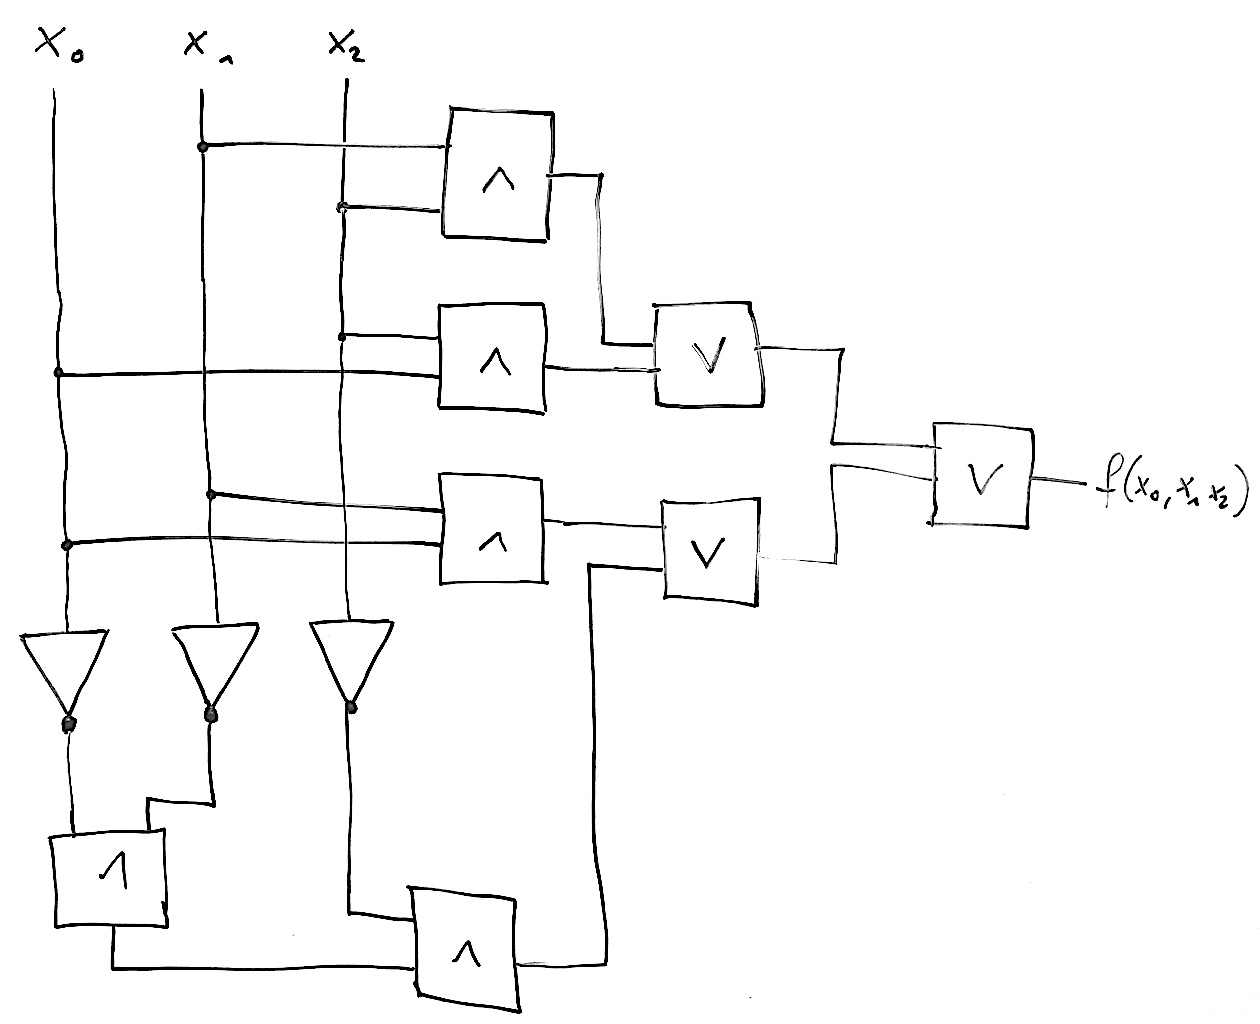
\includegraphics[width=\textwidth]{f.jpeg}
	
		% \begin{circuitikz}[baseline=(current bounding box.north), label distance=2mm]
		% 	\ctikzset{logic ports=ieee,
		% 	logic ports/scale=0.7}
		% 	\tikzstyle{branch}=[fill,shape=circle,minimum size=3pt,inner sep=0pt]

		% 	\node (x2) at (0,0) {$x_2$};
		% 	\node (x1) at (0,2) {$x_1$};
		% 	\node (x0) at (0,4) {$x_0$};
		% 	\draw
		% 		(2,-1) node[not port] (not2) {}
		% 		(2,1)  node[not port] (not1) {}
		% 		(2,3)  node[not port] (not0) {};
		% 	\draw
		% 		(7,-4) node[and port] (and4) {}
		% 		(5,-2) node[and port] (and3) {}
		% 		(7,0) node[and port] (and2) {}
		% 		(7,2) node[and port] (and1) {}
		% 		(7,4) node[and port] (and0) {};
		% 	\draw
		% 		(10,0) node[or port] (or2) {}
		% 		(10,2) node[or port] (or1) {};
		% 	\draw
		% 		(12,1) node[or port] (orf) {};
		% 	\node (f) at (14,1) {$f(x_0,x_1,x_2)$};

		% 	\draw 
		% 		(x0) -| (not0.in)
		% 		(x1) -| (not1.in)
		% 		(x2) -| (not2.in);
		% \end{circuitikz}
		\item[b)] Minimierung von $g$: \\\\
		\begin{tikzpicture}[baseline=(current bounding box.south)]
			\foreach \val[count=\i from 1, evaluate=\i as \j using int(\i+1)] in {
				$\overline{x_2 x_1} x_0$,
				$x_2 \overline{x_1 x_0}$,
				$x_2 \overline{x_1} x_0$,
				$x_2 x_1 x_0$
			}
			\node at(0\width, {-(\i-1)*\height})[] (A\i) {\i. \val};

			\foreach \val[count=\i from 1, evaluate=\i as \j using int(\i+1)] in {
				$\overline{x_1}x_0$,
				$x_2 \overline{x_1}$,
				$x_2 x_0$
			}
			\node at(1\width, {-(\i-1)*\height})[] (B\i) {\val};

			\draw 
				(A1.east) edge (B1.west)
				(A3.east) edge (B1.west)
				(A2.east) edge (B2.west)
				(A3.east) edge (B2.west)
				(A3.east) edge (B3.west)
				(A4.east) edge (B3.west);
			
			\draw 
				(B1.south west) rectangle (B1.north east)
				(B2.south west) rectangle (B2.north east)
				(B3.south west) rectangle (B3.north east);
		\end{tikzpicture}\hspace*{0.5cm}
		\begin{circuitikz}[scale=0.7]
			\ctikzset{tripoles/european not symbol=ieee circle}
			\ctikzset{logic ports/scale=0.7}
			\draw (0,0) node[](x2){$x_2$} ++
			(0,-1) node[](x1){$x_1$} ++
			(0,-1) node[](x0){$x_0$};
			
			\draw (x1) to[inline not] ++(2.5,0) -- ++(0,2.5)
			-- ++(0,0) node[and port, anchor=in 2](AND2-1){}
			
			(x2) to[short, -*] ++(2,0) |- (AND2-1.in 1)
			
			(AND2-1.in 2) to[short, -*] ++(0,-0.5) coordinate(tmp) -- (tmp -| AND2-1.out) node[and port, anchor=bin 1](AND1-0){}
			
			(x0) to[short, -*] (x0 -| AND1-0.in 2) -- (AND1-0.in 2)
			
			(AND1-0.out) -- ++(0,0) node[or port, anchor=in 2](OR1){}
			(AND2-1.out) -| (OR1.in 1)
			
			(x1 -| OR1) node[and port](AND2-0){}
			(x2) -| (AND2-0.in 1)
			(x0) -| (AND2-0.in 2)
			
			(x2 -| OR1) ++(2.5,0) node[or port](OR2){}
			(OR1.out) -| (OR2.in 1)
			(AND2-0.out) -| (OR2.in 2)
			(OR2.out) ++(1.5,0)node[](g){$g(x_2,x_1,x_0)$}
			;
		\end{circuitikz}\\\\
		$\Rightarrow g(x_0, x_1, x_2) = \overline{x_1}x_0 + x_2 \overline{x_1} + x_2 x_0$
		
	\end{enumerate}
	\FloatBarrier

	\subsection*{Aufgabe 2: Aiken-Code}
	\begin{enumerate}
		\item[a)] Siehe Tabelle \ref{t:aiken}.
		\begin{table*}[b]
			\centering
			\begin{tabular}{c|cccc|cccc}
				Dezimal & \multicolumn{4}{c}{Binär} & \multicolumn{4}{|c}{Aiken-Code} \\
				$d$ & $x_1$ & $x_2$ & $x_3$ & $x_4$ & $y_1$ & $y_2$ & $y_3$ & $y_4$ \\ \hline
				0   & 0 & 0 & 0 & 0   & 0 & 0 & 0 & 0 \\
				1   & 0 & 0 & 0 & 1   & 0 & 0 & 0 & 1 \\
				2   & 0 & 0 & 1 & 0   & 0 & 0 & 1 & 0 \\
				3   & 0 & 0 & 1 & 1   & 0 & 0 & 1 & 1 \\
				4   & 0 & 1 & 0 & 0   & 0 & 1 & 0 & 0 \\
				5   & 0 & 1 & 0 & 1   & 1 & 0 & 1 & 1 \\
				6   & 0 & 1 & 1 & 0   & 1 & 1 & 0 & 0 \\
				7   & 0 & 1 & 1 & 1   & 1 & 1 & 0 & 1 \\
				7   & 1 & 0 & 0 & 0   & 1 & 1 & 1 & 0 \\
				9   & 1 & 0 & 0 & 1   & 1 & 1 & 1 & 1 \\
				10  & 1 & 0 & 1 & 0   & \multicolumn{4}{c}{n.d.} \\
				11  & 1 & 0 & 1 & 1   & \multicolumn{4}{c}{n.d.} \\
				12  & 1 & 1 & 0 & 0   & \multicolumn{4}{c}{n.d.} \\
				13  & 1 & 1 & 0 & 1   & \multicolumn{4}{c}{n.d.} \\
				14  & 1 & 1 & 1 & 0   & \multicolumn{4}{c}{n.d.} \\
				15  & 1 & 1 & 1 & 1   & \multicolumn{4}{c}{n.d.} \\
			\end{tabular}
			\caption{Vervollständigte Tabelle aus Aufgabe 2a)}
			\label{t:aiken}
		\end{table*}
		\item[b)]
		\begin{align*}
			y_1(x_1,x_2,x_3,x_4) &= \overline{x_1} x_2 \overline{x_3} x_4 + \overline{x_1}x_2 x_3 \overline{x_4} + \overline{x_1} x_2 x_3 x_4 + x_1 \overline{x_2 x_3 x_4} + x_1 \overline{x_2 x_3} x_4 \\
			y_2(x_1,x_2,x_3,x_4) &= \overline{x_1} x_2 \overline{x_3 x_4} + \overline{x_1} x_2 x_3 \overline{x_4} + \overline{x_1}x_2 x_3 x_4 + x_1 \overline{x_2 x_3 x_4} + x_1 \overline{x_2 x_3} x_4 \\
			y_3(x_1,x_2,x_3,x_4) &= \overline{x_1 x_2} x_3 \overline{x_4} + \overline{x_1 x_2} x_3 x_4 + \overline{x_1} x_2 \overline{x_3} x_4 + x_1 \overline{x_2 x_3 x_4} + x_1 \overline{x_2 x_3} x_4 \\
			y_4(x_1,x_2,x_3,x_4) &= \overline{x_1 x_2 x_3} x_4 + \overline{x_1 x_2} x_3 x_4 + \overline{x_1} x_2 \overline{x_3} x_4 + \overline{x_1} x_2 x_3 x_4 + x_1 \overline{x_2 x_3} x_4 
		\end{align*}
		\item[c)] Siehe Abbildung \ref{f:minimierung}.
		\begin{figure}[ht]
			\begin{minipage}[b]{0.5\linewidth}
				\centering
				$y_1(x_1,x_2,x_3,x_4)$:\\ \vspace*{1em}
				\begin{kvmap}
					\begin{kvmatrix}{x_2,x_4,x_1,x_3}
						0 & 0 & 1 & 0 \\
						0 & 0 & 1 & 1 \\
						* & * & * & * \\
						1 & 1 & * & * 
					\end{kvmatrix}
					\bundle[color=red]{2}{0}{2}{3}
					\bundle[color=green]{0}{2}{3}{3}
					\bundle[color=blue]{2}{1}{3}{2}
				\end{kvmap}\\ \vspace*{1em}
				$\Rightarrow y_1(x_1,x_2,x_3,x_4) = x_1 + x_2 x_4 + x_2 x_3$
			\end{minipage}\vline
			\begin{minipage}[b]{0.5\linewidth}
				\centering
				$y_2(x_1,x_2,x_3,x_4)$:\\ \vspace*{1em}
				\begin{kvmap}
					\begin{kvmatrix}{x_2,x_4,x_1,x_3}
						0 & 0 & 0 & 1 \\
						0 & 0 & 1 & 1 \\
						* & * & * & * \\
						1 & 1 & * & * 
					\end{kvmatrix}
					\bundle[color=red]{3}{0}{3}{3}
					\bundle[color=green]{0}{2}{3}{3}
					\bundle[color=blue]{2}{1}{3}{2}
				\end{kvmap}\\ \vspace*{1em}
				$\Rightarrow y_2(x_1,x_2,x_3,x_4) = x_1 + x_2 \overline{x_4} + x_2 x_3$
			\end{minipage}\\
			\vspace*{1em}
			\rule{\linewidth}{0.4pt}\\
			\begin{minipage}[b]{0.5\linewidth}
				\centering
				$y_3(x_1,x_2,x_3,x_4)$:\\ \vspace*{1em}
				\begin{kvmap}
					\begin{kvmatrix}{x_2,x_4,x_1,x_3}
						0 & 0 & 1 & 0 \\
						1 & 1 & 0 & 0 \\
						* & * & * & * \\
						1 & 1 & * & * 
					\end{kvmatrix}
					\bundle[color=red, invert=true]{2}{3}{2}{0}
					\bundle[color=green]{0}{2}{3}{3}
					\bundle[color=blue]{0}{1}{1}{2}
				\end{kvmap}\\ \vspace*{1em}
				$\Rightarrow y_3(x_1,x_2,x_3,x_4) = x_1 + x_2 \overline{x_3} x_4 + \overline{x_2} x_3$
			\end{minipage}\vline
			\begin{minipage}[b]{0.5\linewidth}
				\centering
				$y_4(x_1,x_2,x_3,x_4)$:\\ \vspace*{1em}
				\begin{kvmap}
					\begin{kvmatrix}{x_2,x_4,x_1,x_3}
						0 & 1 & 1 & 0 \\
						0 & 1 & 1 & 0 \\
						* & * & * & * \\
						0 & 1 & * & * 
					\end{kvmatrix}
					\bundle[color=green]{1}{0}{2}{3}
				\end{kvmap}\\ \vspace*{1em}
				$\Rightarrow y_4(x_1,x_2,x_3,x_4) = x_4$
			\end{minipage}
			\caption{Minimierte Schaltfunktionen}
			\label{f:minimierung}
		\end{figure}
		\item[d)] Da die Funtionen mittels KV minimiert wurden, liegen sie in orthogonaler Form vor. Daher können die OR-Verknüpfungen einfach dur XOR ersetzt werden. Anschließend müssen die Komplemente noch in der Form $\overline{a} = a \oplus 1$ dargestellt werden. 
		\begin{align*}
			y_1(x_1,x_2,x_3,x_4) &= x_1 \oplus x_2 x_4 \oplus x_2 x_3 \\
			y_2(x_1,x_2,x_3,x_4) &= x_1 \oplus x_2 \overline{x_4} \oplus x_2 x_3 = x_1 \oplus x_2 (x_4 \oplus 1) \oplus x_2 x_3 \\
			y_3(x_1,x_2,x_3,x_4) &= x_1 \oplus x_2 \overline{x_3} x_4 \oplus \overline{x_2} x_3 = x_1 \oplus x_2 (x_3 \oplus 1) x_4 \oplus (x_2 \oplus 1) x_3 \\
			y_4(x_1,x_2,x_3,x_4) &= x_4
		\end{align*}
		Die Schaltfunktionen sind in Abbildung \ref{f:aiken} dargestellt.
		\begin{figure}[h]
			\centering
			\begin{circuitikz}
				\ctikzset{tripoles/european not symbol=ieee circle}
				\draw (0,0) node[](x1){$x_1$} ++
				(0,-2) node[](x2){$x_2$} ++
				(0,-2) node[](x3){$x_3$} ++
				(0,-2) node[](x4){$x_4$}
				
				(x3) -- ++(2,0) to[short, *-] ++(0,0.75) node[and port, anchor=in 2](AND23){}
				(x2) to[short, -*] (x2 -| AND23.in 1) -- (AND23.in 1)
				
				(x4) -- ++(1,0) to[short, *-] ++(0,0.75) coordinate(tmp) -- (tmp -| AND23.in 1) node[and port, anchor=in 2](AND24){}
				(x2) to[short, -*] ++(1,0) |- (AND24.in 1)
				
				(AND23.out) to[short, -*] ++(0.5,0) node[and port, anchor=in 1](AND234){}
				(x4) to[short, -*] (x4 -| AND234.in 2) -- (AND234.in 2)
				
				(x1) -- (x1 -| AND234.in 1) node[xor port, anchor=in 1](XOR1){}
				(AND23) -| (XOR1.in 2)
				(XOR1.out) -- ++(0.5,0) node[xor port, anchor=in 1](XOR2){}
				(AND24.out) -| (XOR2.in 2)
				(XOR2.out) to[short, -*] ++(2,0) coordinate(tmp) -- ++(3,0) coordinate(out) node[right](){$y_1$}
				
				(x2) -- (x2 -| tmp) node[xor port, anchor=in 2](XOR3){}
				(XOR3.out) -- (XOR3 -| out) node[right](){$y_2$}
				
				(AND234.out) -- (AND234 -| XOR2.bout) node[xor port, anchor=bin 1](XOR4){}
				(x3) -| (XOR4.in 2)
				(XOR4.out) -- (XOR4 -| tmp) node[xor port, anchor=in 2](XOR5){}
				(XOR5.out) -- (XOR5 -| out) node[right](){$y_3$}
				
				(tmp) to[short, -*] (XOR3.in 1 -| tmp) -- (XOR5.in 1 -| tmp)
				
				(x4) -- (x4 -| out) node[right](){$y_4$}
				;
			\end{circuitikz}
			\caption{Aiken-Code Schaltung}
			\label{f:aiken}
		\end{figure}

		% \begin{figure}[h]
		% 	\centering
		% 	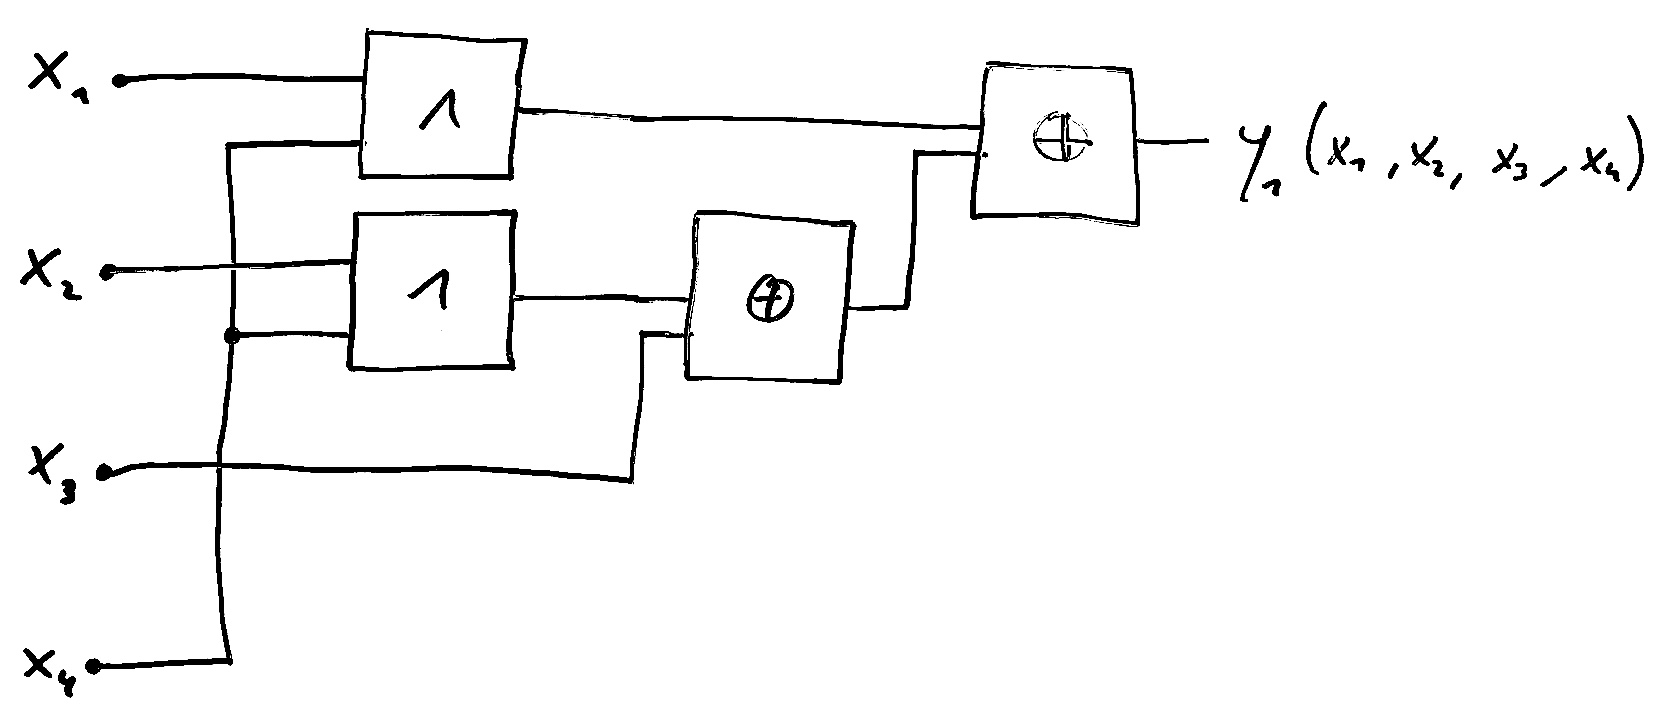
\includegraphics[scale=.17]{y1.jpeg}
		% 	\caption{$y_1(x_1,x_2,x_3,x_4)$}
		% 	\label{f:y1}
		% \end{figure}
		% \begin{figure}[h]
		% 	\centering
		% 	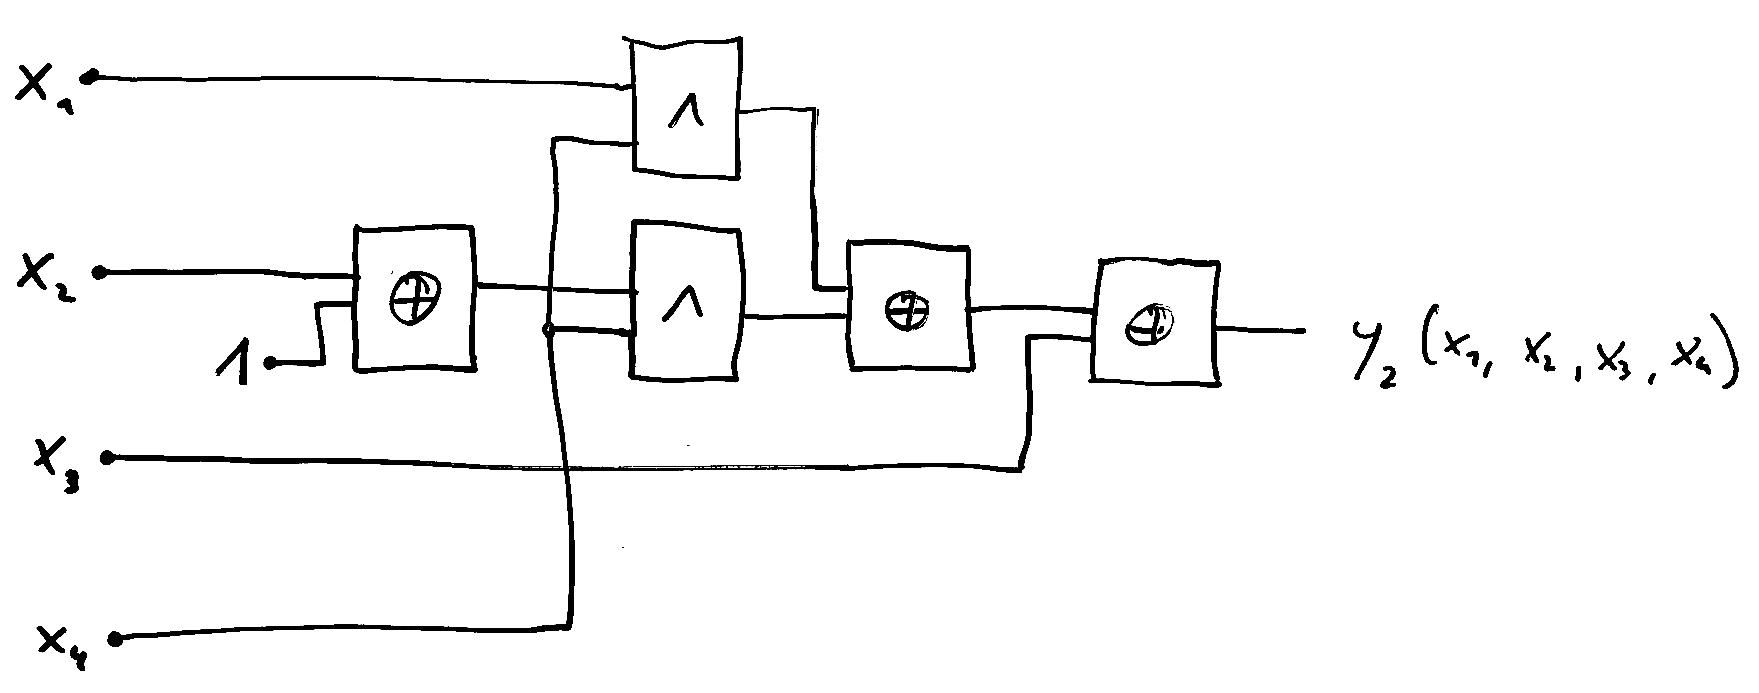
\includegraphics[scale=.17]{y2.jpeg}
		% 	\caption{$y_2(x_1,x_2,x_3,x_4)$}
		% \end{figure}
		% \begin{figure}[h]
		% 	\centering
		% 	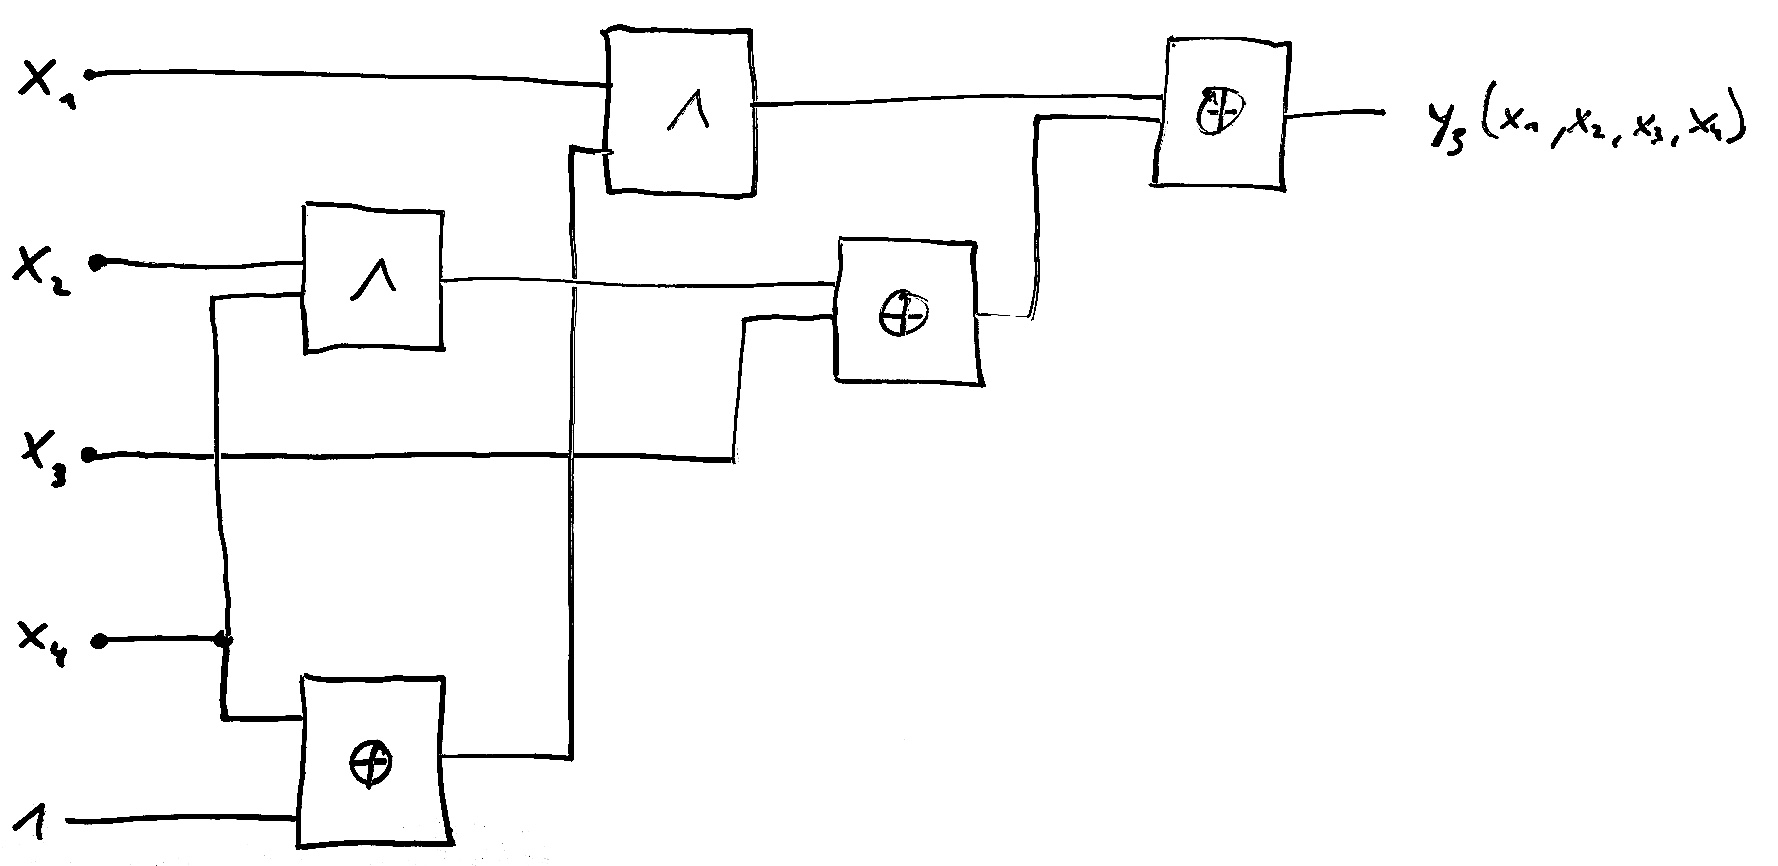
\includegraphics[scale=.17]{y3.jpeg}
		% 	\caption{$y_3(x_1,x_2,x_3,x_4)$}
		% \end{figure}
		% \begin{figure}[h]
		% 	\centering
		% 	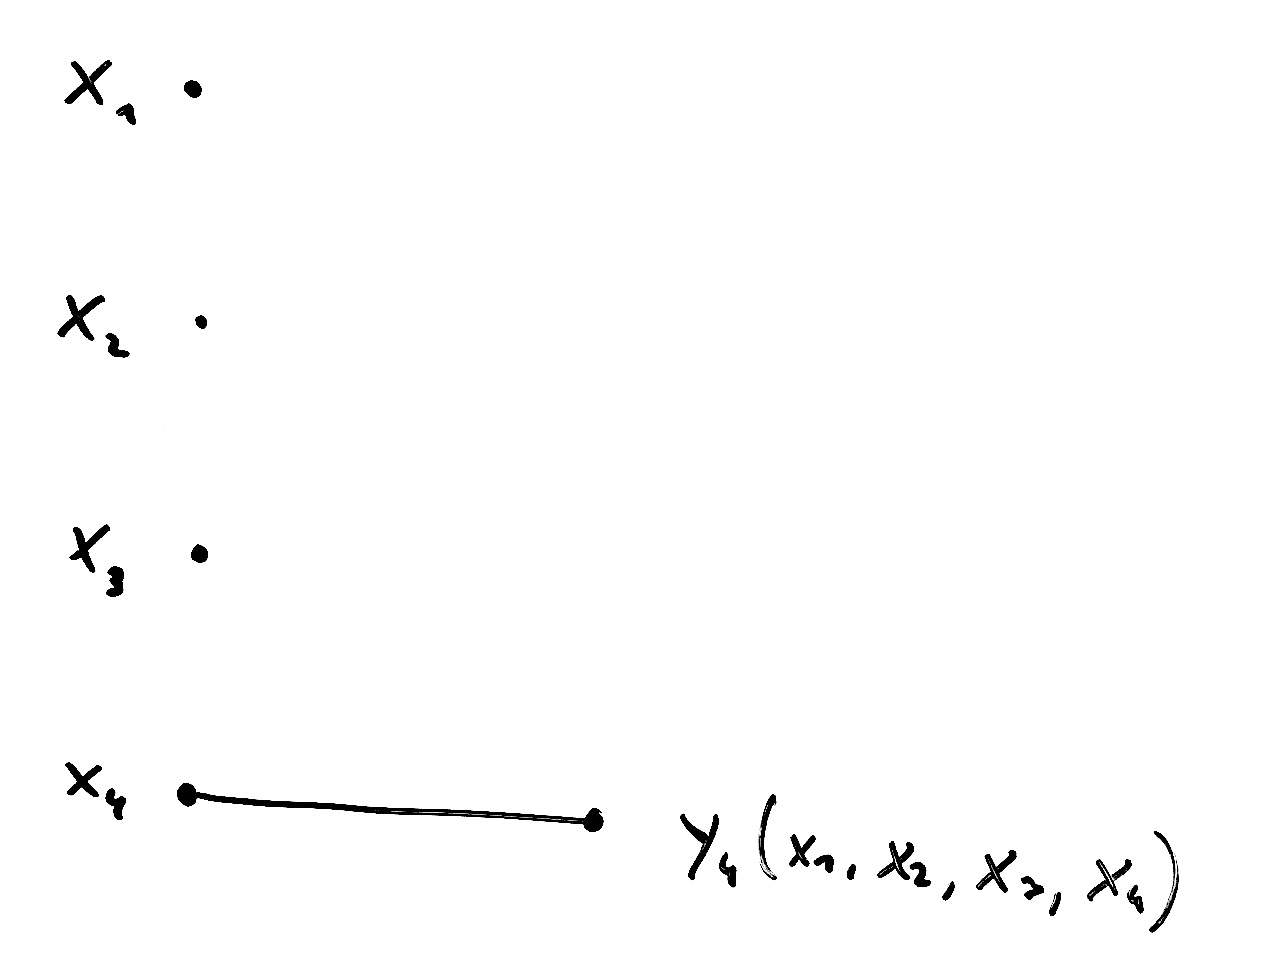
\includegraphics[scale=.17]{y4.jpeg}
		% 	\caption{$y_4(x_1,x_2,x_3,x_4)$}
		% 	\label{f:y4}
		% \end{figure}
		% \begin{circuitikz}[baseline=(current bounding box.north), label distance=2mm]
		% 	\ctikzset{
		% 		logic ports=ieee,
		% 		logic ports/scale=0.7
		% 	}
		% 	\draw
		% 		node [anchor=east] (x4) at (0,0) {$x_4$}
		% 		node [anchor=east] (x3) at (0,2) {$x_3$}
		% 		node [anchor=east] (x2) at (0,4) {$x_2$}
		% 		node [anchor=east] (x1) at (0,6) {$x_1$}
		% 		node [anchor=west] (y)  at (7,2) {$y_3$}
				
		% 		node [and port, anchor=in 1] (and2) at (2,3) {}
		% 		node [and port, anchor=in 1] (and1) at (2,6) {}
		% 		node [or port, anchor=in 2] (or1) at (4.5,and2.out) {}
		% 		node [or port, anchor=in 2] (or2) at (5.5,2) {}
				
		% 		(and1.out) -| (or1.in 1)
		% 		(and2.out) -| (or1.in 2)
		% 		(or1.out) -| (or2.in 1)
		% 		(or2.out) -| (y.west)
		% 		(x3) -| (or2.in 2)
		% 		(x1) -| (and1.in 1)
		% 		(x4) |- (and1.in 2)
		% 		;
		% \end{circuitikz}
		
		% \begin{circuitikz}[baseline=(current bounding box.north), label distance=2mm]
		% 	\ctikzset{
		% 		logic ports=ieee,
		% 		logic ports/scale=0.7
		% 	}
		% 	\node (x4) at (0,0) {$x_4$};
		% 	\node at (x4.east) {\textbullet};
		% 	\node (out) at (3,0) {$y_4$};
		% 	\node at (out.west) {\textbullet};
		% 	\draw (x4.east) |- (out.west);

		% \end{circuitikz}

	\end{enumerate}
	\FloatBarrier

	\subsection*{Aufgabe 3: RS-Flipflop}
	\begin{enumerate}
		\item[a)] Der $R$-Eingang ist der "`Reset"'-Eingang. Wird dort eine logische 1 angelegt, stellt sich der Ausgang $Q$ stets auf 0 um - egal ob dort vorher eine 1 stand, oder nicht. Umgekehrt entsteht durch eine logische 1 an Eingang $S$ stets eine 0 am Ausgang $Q$, unabhängig davon, was dort vorher gespeichert war. Wird keiner der beiden Eingänge betätigt, bleibt der Ausgang in $Q$ gespeichert. Somit kann in einem RS-Flipflop 1 Bit Information dauerhaft gesichert werden. 
		
		Betägtigt man gleichzeitig zu $S = R = 1$, gelangt man in den "`verbotenen"' Zustand. Im Falle eines NOR-RS-Flipflop entsteht dann an beiden Ausgängen eine logische 0, im Falle eines NAND-RS-Flipflop entsteht an beiden Ausgängen eine logische 1. Lässt man beide Eingänge im selben Moment los, gelangt man theoretisch in den "`metastabilen"' Zustand. In der Praxis entsteht aufgrund minimaler Zeitdifferenzen ein beliebiger Ausgang - das Resultat ist undefiniert. 
		\item[b)/c)] Siehe Abbildung \ref{f:rs_flipflop}.
		\begin{figure}[h]
			\begin{subfigure}[b]{0.5\linewidth}
				\centering
				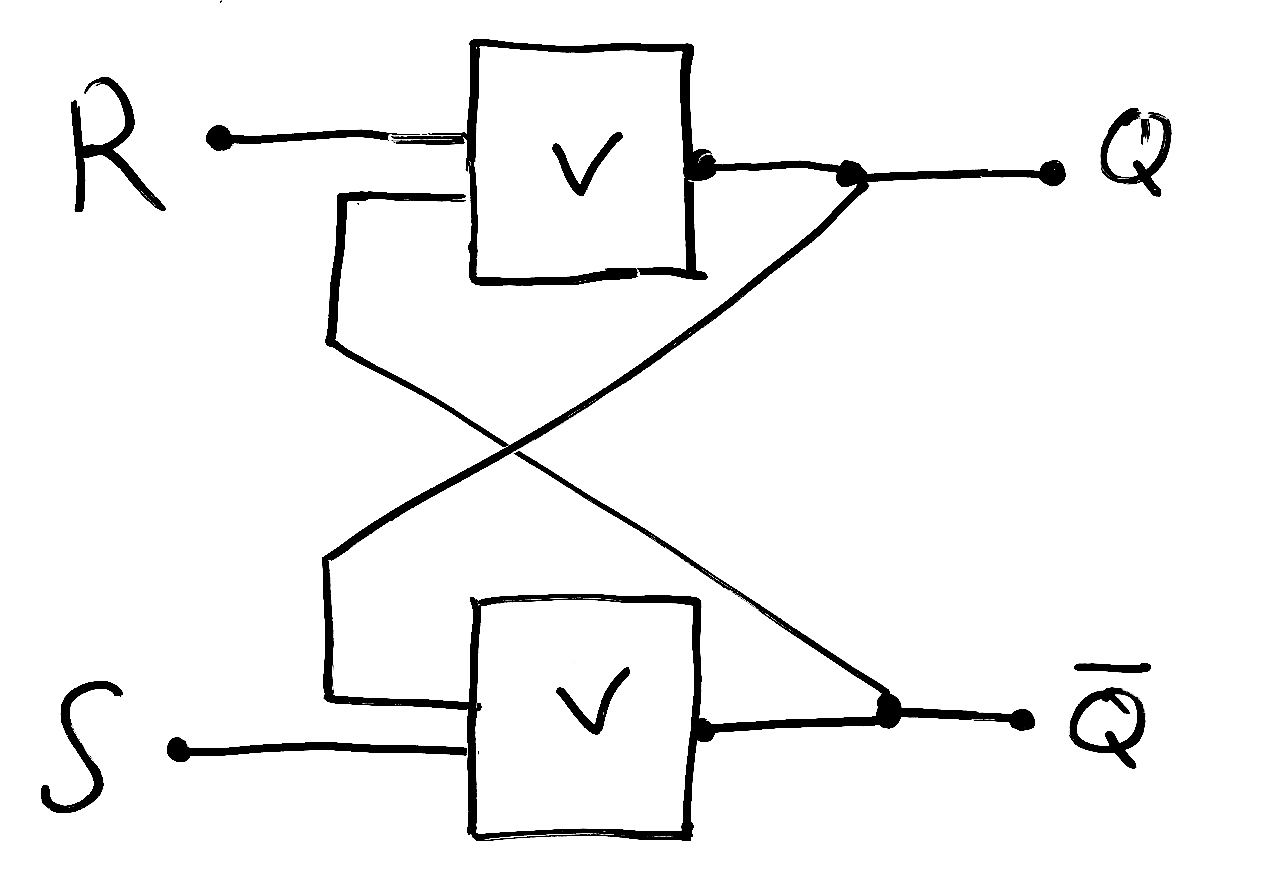
\includegraphics[width=.8\linewidth]{nor_rs.jpeg}
				\caption{NOR-RS-Flipflop}
				\label{f:nor_rs}
			\end{subfigure}
			\begin{subfigure}[b]{0.5\linewidth}
				\centering
				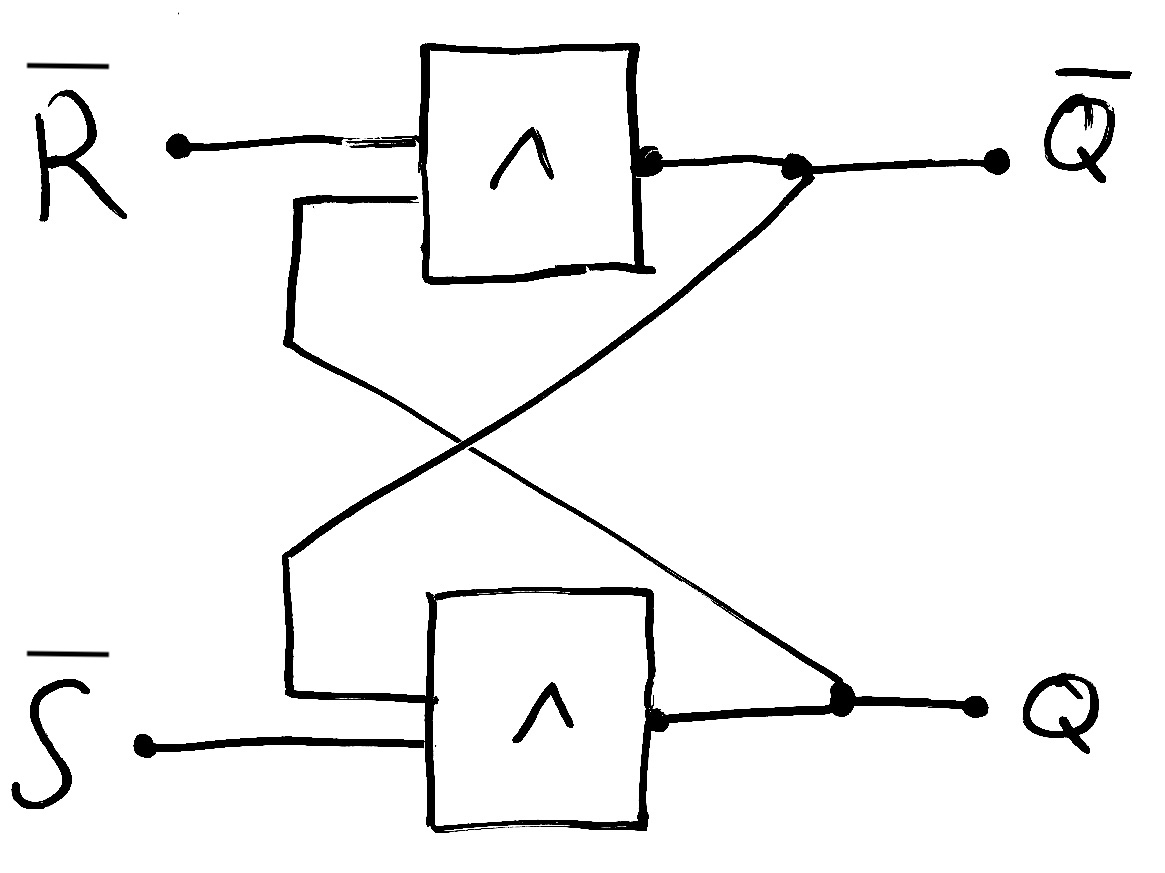
\includegraphics[width=.8\linewidth]{nand_rs.jpeg}
				\caption{NAND-RS-Flipflop}
				\label{f:nand_rs}
			\end{subfigure}
			\caption{RS-Flipflop}
			\label{f:rs_flipflop}
		\end{figure}
		\item[d)] Siehe Abbildung \ref{f:signal_rs}.
		\begin{figure}[h]
			\centering
			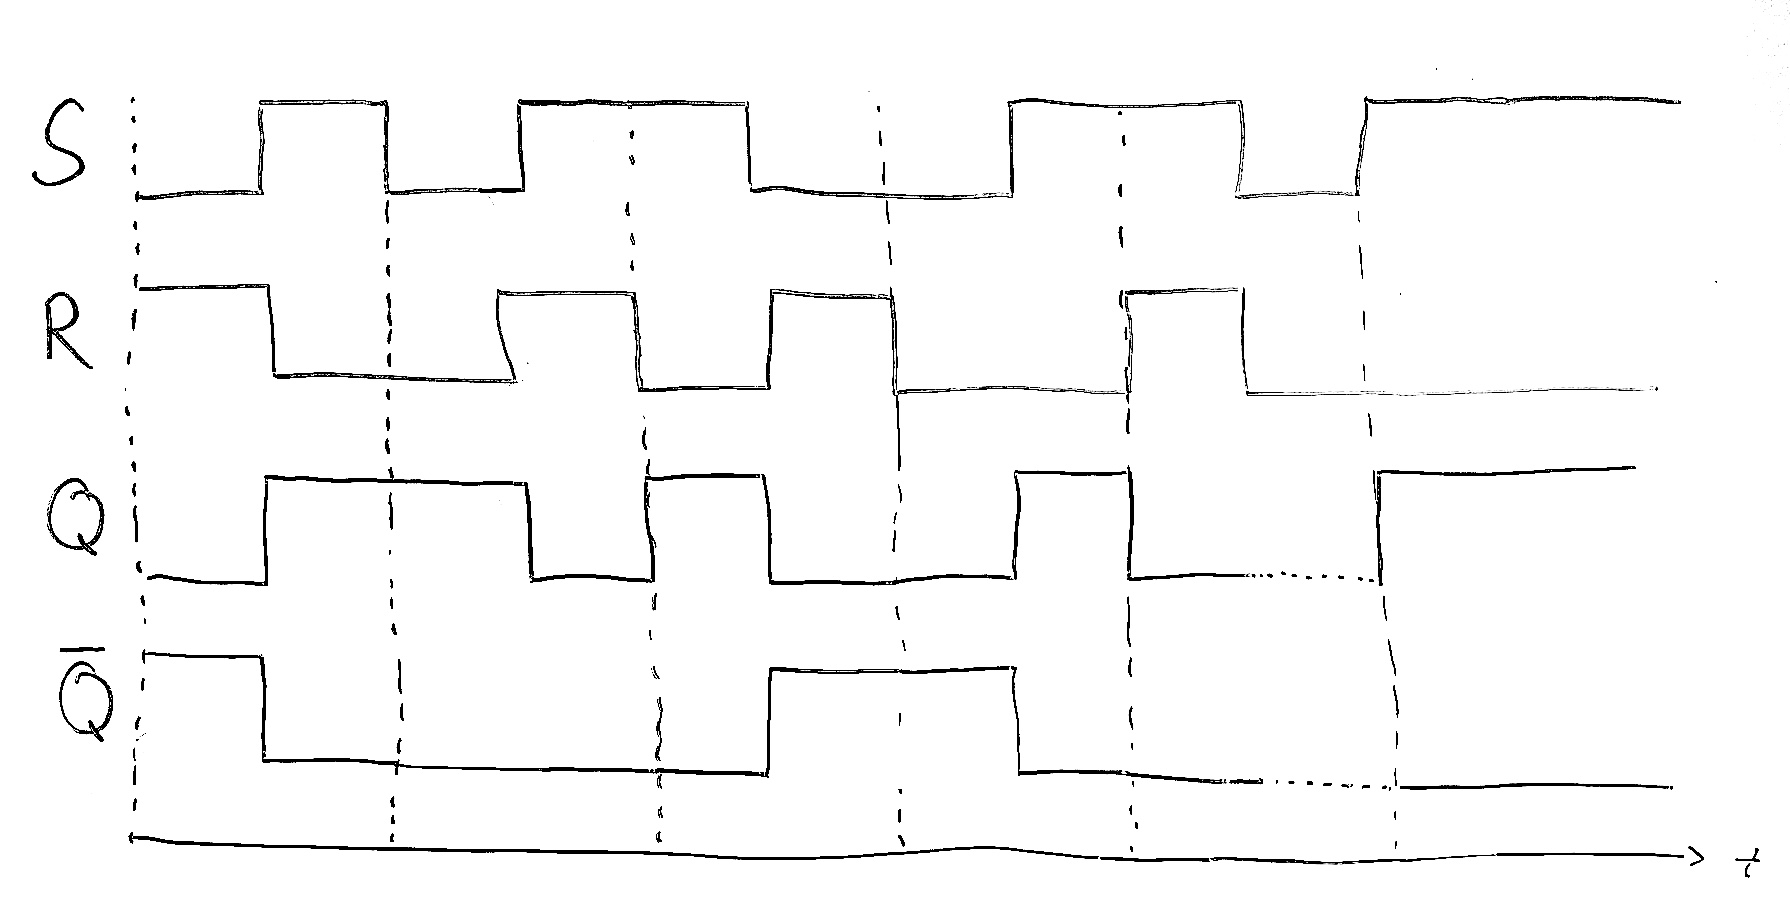
\includegraphics[width=\linewidth]{signalverlauf_rs.jpeg}
			\caption{Signalverlauf RS-FF (Gezeigt ist der Verlauf eines NOR-RS-Flipflop)}
			\label{f:signal_rs}
		\end{figure}
	\end{enumerate}
	\FloatBarrier

	\subsection*{Aufgabe 4: D-FF und D-Latch}
	\begin{enumerate}
		\item[a)] Siehe Abbildung \ref{f:dlff}
		\begin{figure}[h]
			\centering
			\begin{subfigure}[b]{0.45\linewidth}
				\centering
				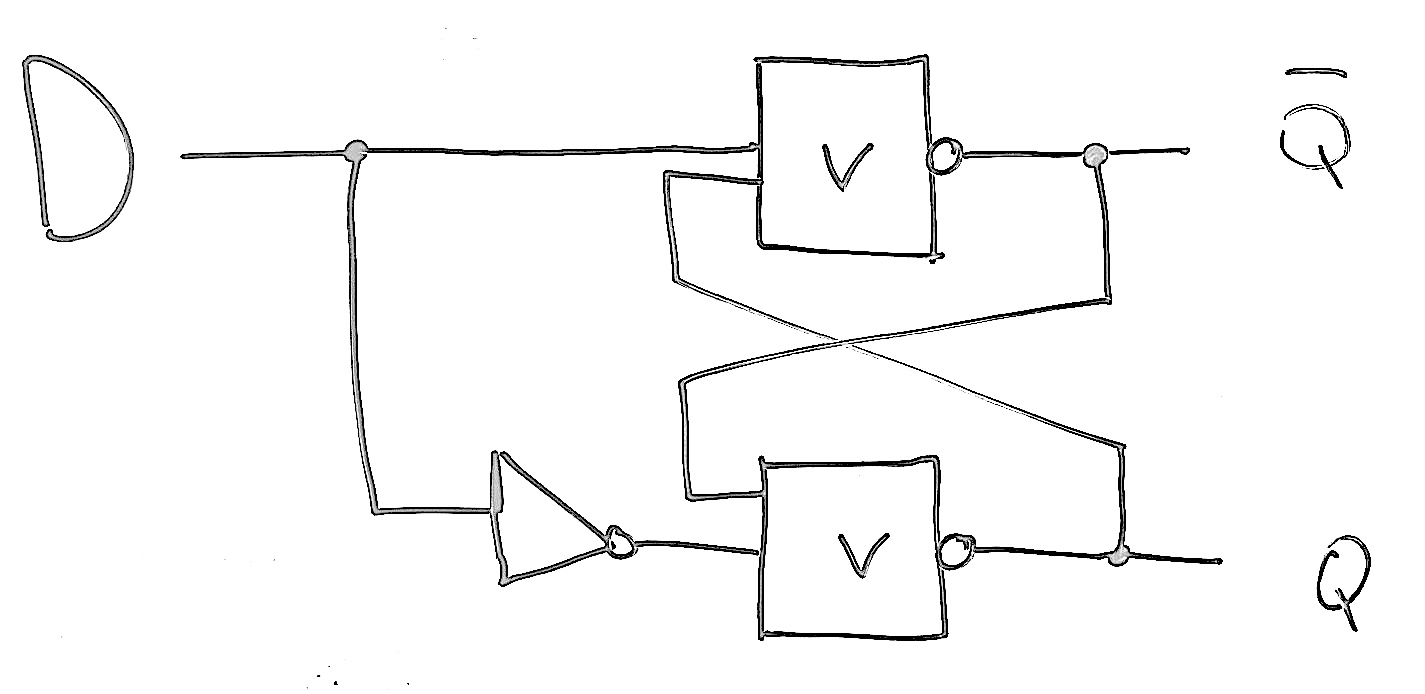
\includegraphics[width=.8\linewidth]{dlatch.jpeg}
				\caption{D-Latch}
				\label{f:dlatch}
			\end{subfigure}
			\begin{subfigure}[b]{0.45\linewidth}
				\centering
				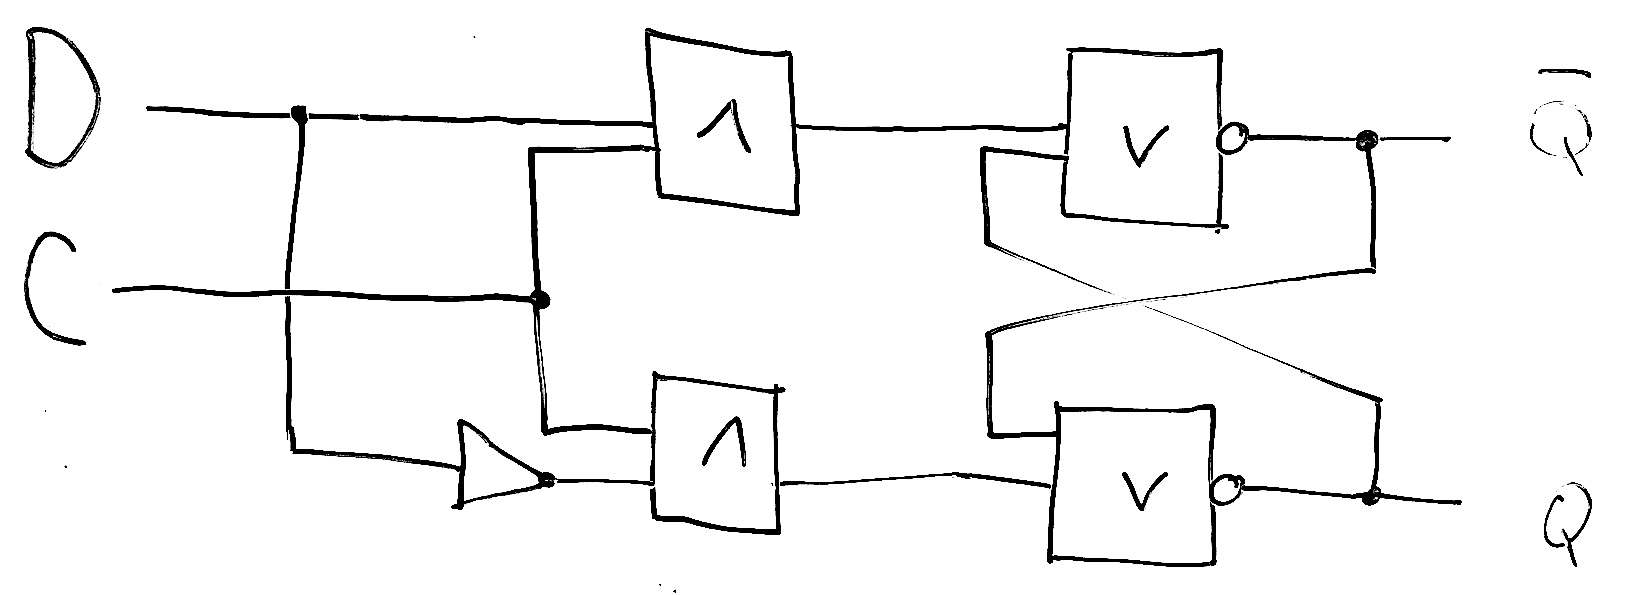
\includegraphics[width=\linewidth]{dff.jpeg}
				\caption{Positiv taktzustandsgesteuerter D-Flipflop}
				\label{f:dff}
			\end{subfigure}
			\caption{D-Latch und D-FF}
			\label{f:dlff}
		\end{figure}
		\item[b)] Beim D-Latch bzw. D-FF steht das "`D"' für \textit{Data}. Will man also eine 1 speichern, liegt an D eine 1 an - will man eine 0 speichern, liegt eine 0 an. Dadurch, dass nur dieser eine Input (und sein Komplement) vorliegt, kann auch nie der verbotene Zustand erreicht werden. 

		Der D-FF ist eine Erweiterung des D-Latch: Er erlaubt einen Wechsel des gespeicherten Zustands nur, wenn auch das Control-Signal "`C"' aktiv ist. Ansonsten verharrt der D-FF im Hold-Zustand. Der Vorteil dabei ist, dass der D-Eingang nicht ständig auf der gewünschten 1 oder 0 gehalten werden muss, sondern beliebige Werte annehmen kann, solange nicht auch der Control-Eingang aktiviert wird. Im D-FF kann somit dauerhaft ein Zustand gespeichert werden und ggf. durch Aktivierung des Control-Eingangs verändert werden. 
		\item[c)] Siehe Abbildung \ref{f:signalverlauf_dff}.
		\begin{figure}[h]
			\centering
			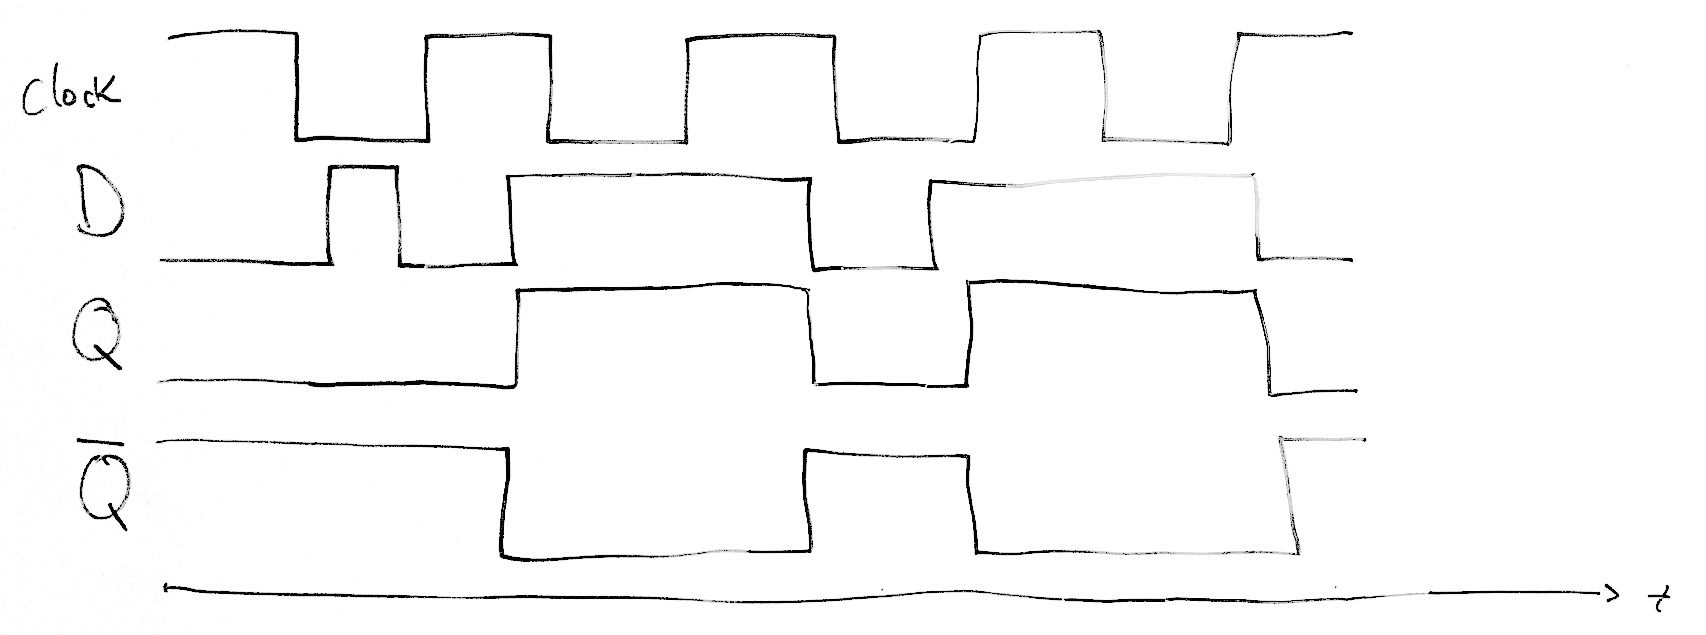
\includegraphics[width=\linewidth]{signalverlauf_dff.jpeg}
			\caption{Signalverlauf D-FF}
			\label{f:signalverlauf_dff}
		\end{figure}
		 
	\end{enumerate}

\end{document}